\section{Requirements Specification}\label{sec:requirements-specification}

\subsection{Functional Requirements}\label{subsec:functional-requirements}
The system provides comprehensive functionality in three main areas: \textbf{Basic Calendar Features}, \textbf{Additional Calendar Features}, \textbf{Secure Interactions}.

Under the \textbf{Basic Calendar Features} category, the system offers weekly and daily views, with filtering capabilities by room and user.
The system allows managers to create, edit, and delete events, while users can only view the calendar and search for resource availability.

In the \textbf{Additional Calendar Features} category, the system offers a day view, which displays events for a specific day organized by room.
Furthermore, the system offers a \texttt{FindAvailable} feature, which allows users to search for available resources (rooms, users, or events) based on various criteria.

Under the \textbf{Secure Interactions} category, the system offers a login system, which allows users to log into the system using a username and password.
The system stores all passwords in a hashed format using the BCrypt algorithm.
Instead of traditional session-based authentication, the system uses JWT tokens to authenticate users stateless-way.
This method was learned from the video resource~\cite{Amigoscode2023}.

\subsection{Non-Functional Requirements}\label{subsec:non-functional-requirements}

The application prioritizes function over design by providing a simple and intuitive user interface.
Navigation and interaction patterns remain consistent throughout the system, with clear error messages and feedback mechanisms to guide users.

Security is implemented through JWT-based authentication, with all communication restricted to HTTPS. The system incorporates protection against common web vulnerabilities and maintains strict access controls.

Reliability is ensured through robust error handling and data consistency mechanisms.

Maintainability is supported by comprehensive documentation, a modular architecture, and extensive test coverage.
This ensures that the system can be easily updated and maintained over time.


\section{System Architecture}\label{sec:system-architecture}

\subsection{Overall Architecture}\label{subsec:overall-architecture}
The application follows a four-tier architecture pattern, separating concerns across \texttt{Models}, \texttt{Views}, \texttt{Controllers}, and the \texttt{Database}.
This~\ref{fig:architecture} separation enables better maintainability and scalability while keeping the system modular and efficient.

\begin{figure}[h]
    \centering
    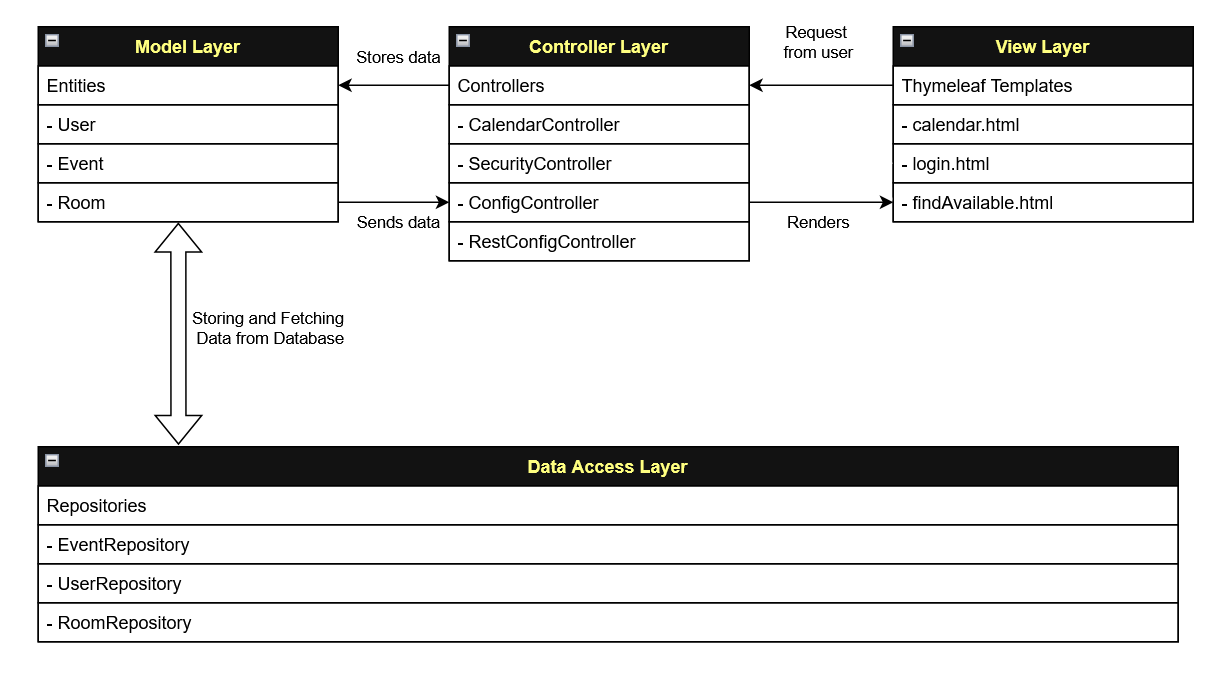
\includegraphics[width=0.8\textwidth]{MVCSchema}
    \caption{System Architecture Diagram}
    \label{fig:architecture}
\end{figure}

\subsection{Key Components}\label{subsec:key-components}

The front-end components utilize Thymeleaf templates for server-side rendering, enhanced with JavaScript for client-side interactivity and CSS for design.
This combination provides a modern, dynamic user experience while maintaining performance, as the Thymeleaf templates are rendered on the server side.

The backend architecture consists of controllers handling HTTP requests and responses, services implementing business logic, repositories managing data access, and a comprehensive security layer handling authentication and authorization.

\subsection{API Design}\label{subsec:api-design}

The application provides both REST API endpoints and view-based endpoints to support various client needs.
The REST API follows standard conventions and provides endpoints for authentication, resource management, and system queries.

Authentication endpoints handle user sign-in, registration, and logout operations.
Resource endpoints manage rooms and events, while query endpoints provide functionality to check resource availability and validate authentication tokens.

View endpoints serve the user interface, with dedicated routes for calendar views and system configuration.
Calendar views support weekly and daily perspectives, while configuration views provide interfaces for managing rooms, events, and users.

The basics of this design were adopted following guidance from the video resource~\cite{VisualComputerScience2023}.


\section{Database Design}\label{sec:database-design}

\subsection{Database Schema}\label{subsec:database-schema}
The database schema~\ref{fig:schemaDB} is designed around three main entities: users, rooms, and events.

After that, the \texttt{roles} table is used to manage the user roles.

In addition, 3 tables of \texttt{tags} are used to manage the tags for rooms, events, and users to simplify the search for resources.

\begin{figure}[h]
    \centering
    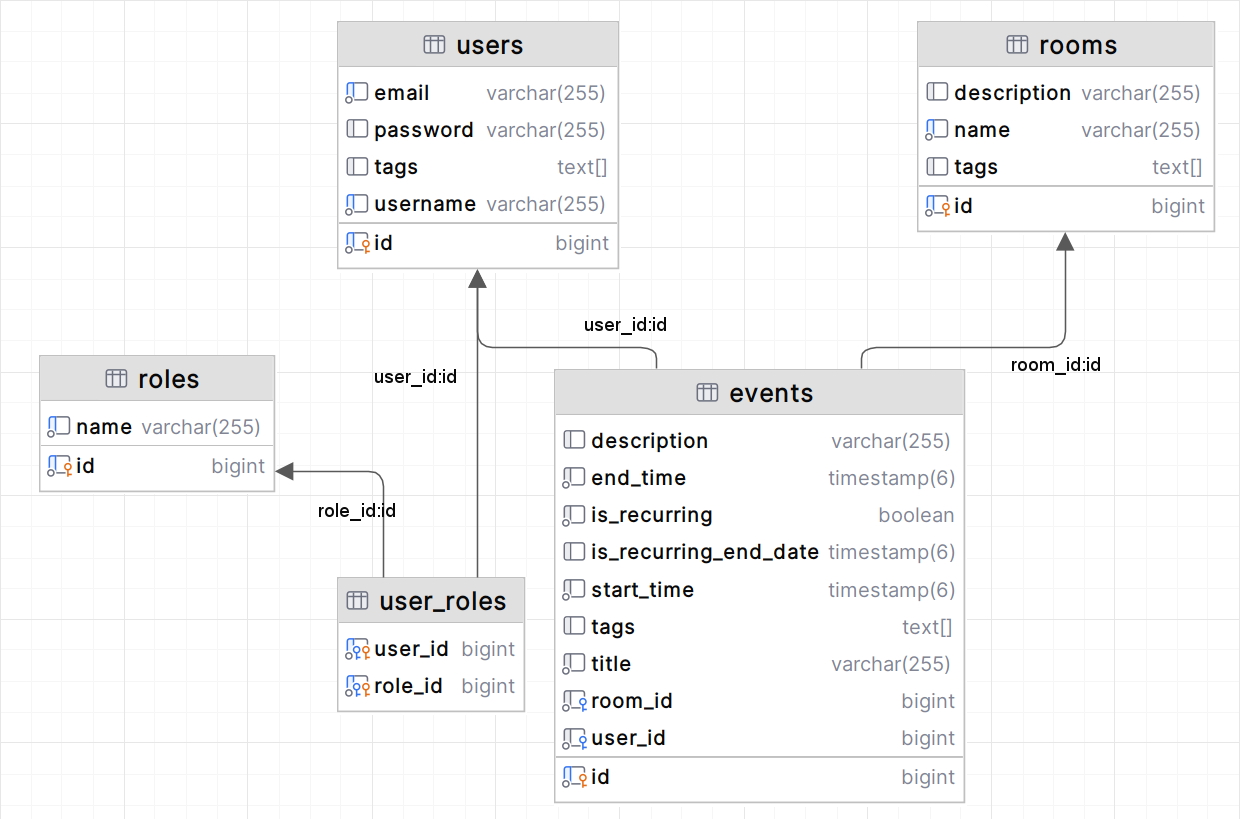
\includegraphics[width=1\textwidth]{schemaDB}
    \caption{Database Schema Diagram}
    \label{fig:schemaDB}
\end{figure}

\subsection{Key Tables and Relationships}\label{subsec:key-tables}

The table ``users'' stores essential user information, including username, email, and securely hashed passwords.
Maintains a many-to-many relationship with the role table, enabling flexible role assignment and management.
This solution is not the most elegant one, as it requires additional queries to get the roles of a user.
However, it was chosen to simplify the implementation of authentication and authorization.

The roles table defines the various user roles within the system, with a connection to the users table using another table called \texttt{user\_roles}.
This design allows for the easy addition of new roles and modification of existing role permissions.

The room table contains information about spaces, including names, descriptions, and categorization tags.
Creating a one-to-many relationship with the events table, the rooms table can have multiple events, but not at the same time.

The event table serves as the central scheduling entity, storing event details such as title, description, timing information, and recurrence settings.
Events maintain relationships with both users and rooms, tracking who is involved and where the event takes place.
Recurrence is implemented following the RFC 5545 standard\cite{rfc5545}.

\subsection{Spring Data JPA Implementation}\label{subsec:spring-data-jpa}

The application relies on Spring Data JPA for efficient data persistence.
Entity classes are annotated with @Entity and @Table, while repositories extend JpaRepository to provide standard CRUD operations.
Relationships between entities are managed through JPA annotations and Spring handles transaction management automatically.
The method of implementing the relationships was learned from the spring.io wiki~\cite{SpringDataJPA2024}.

\section{User Interface Design}\label{sec:ui-design}

\subsection{Design Philosophy}\label{subsec:design-philosophy}
The design of the user interface emphasizes simplicity, consistency, responsiveness, and accessibility.


% Converted HSL→RGB→hex (approximate)
\definecolor{colorGold}{HTML}{F9E14D}       % from HSL(46.8,92.9,61.6)
\definecolor{colorSecondary}{HTML}{C78094}  % HSL(336,25,60)
\definecolor{colorTertiary}{HTML}{772852}   % HSL(314,53,21)
\definecolor{colorAccent}{HTML}{662640}     % HSL(339,27,17)
\definecolor{colorAdditional}{HTML}{0B0A0A}% HSL(345,18,4)

The main colors are
\begin{itemize}
    \item \textcolor{colorGold}{\textbf{--color-gold} (46.8\%, 92.9\%, 61.6\%): Gold}
    \item \textbf{--color-primary} (0\%, 0\%, 100\%): White
    \item \textcolor{colorSecondary}{\textbf{--color-secondary} (336\%, 25\%, 60\%): Dusty Rose}
    \item \textcolor{colorTertiary}{\textbf{--color-tertiary} (314\%, 53\%, 21\%): Deep Magenta}
    \item \textcolor{colorAccent}{\textbf{--color-accent} (339\%, 27\%, 17\%): Plum}
    \item \textcolor{colorAdditional}{\textbf{--color-additional} (345\%, 18\%, 4\%): Charcoal}
\end{itemize}

\subsection{Key Interface Components}\label{subsec:interface-components}

The calendar view presents a weekly grid layout with color-coded events.

Event management features include forms to create and edit events, quick filters for different event types, and clear conflict warnings.
The interface guides users through the event creation process while preventing scheduling conflicts.

Navigation is streamlined through a consistent menu structure.
